\section{AJ-RNN}
``Adversarial Joint-Learning Recurrent Neural Network for Incomplete Time Series Classification" \cite{ajrnn} is a research paper that proposes a novel approach for classification of incomplete time series data.
The authors begin by highlighting the challenges of working with incomplete time series data, particularly the difficulty of extracting features and the need to deal with missing values.

To address these challenges, the authors propose an adversarial joint-learning recurrent neural network (AJ-RNN) that uses a recurrent neural network (RNN) to capture the temporal dependencies in the time series data, and an adversarial learning approach to impute the missing values.

The AJ-RNN is trained using a joint optimization framework that alternates between training the RNN for classification and the imputation network to fill in the missing values.
The adversarial component of the imputation network is used to ensure that the imputed values are as close as possible to the true values.

The authors evaluate the performance of the AJ-RNN on several real-world datasets and demonstrate that it outperforms several existing state-of-the-art approaches for time series classification.

\subsection{Adversarial learning}

% TODO review
Previous studies have shown that adversarial approaches outperform traditional methods in generating data that conforms to the distribution of a given dataset \cite{goodfellow2014generative, ledig2017photo}.

Furthermore, GANs have shown promising results in filling in missing data in time series prediction \cite{yoon2018gain, li2018learning, luo2018multivariate}. Similarly, adversarial techniques have also been applied to tasks such as video captioning \cite{yang2018video} and domain adaptation \cite{ganin2017domain}.
However, prior to this paper, the question of how to apply adversarial learning in the domain of incomplete time series classification (ITSC) has not been explored.

The integration of adversarial training and joint learning in recurrent neural networks (RNNs) is explored in this paper, resulting in the development of a system called Adversarial Joint learning RNN (AJ-RNN).

The study's results show that employing AJ-RNN, an end-to-end framework integrating adversarial training and joint learning in recurrent neural networks, is an effective solution to tackle the issue of incomplete time series classification.
AJ-RNN is trained to predict the value of the next input variable when it is revealed, and to fill in the missing value with its prediction.
At the same time, AJ-RNN also learns to classify.
Hence AJ-RNN can directly perform classification with missing values.

\subsection{Model}


The following section presents the Adversarial Joint learning Recurrent Neural Network (AJ-RNN) as a solution for time series classification with missing values. 
The architecture of the model is illustrated in Figure \ref{fig:AJRNNrchitecture}. 

Here we describe how adversarial and joint learning strategies are integrated into an RNN.


The time series $X$ is represented as a sequence vector of $T$ observations, denoted by $X = \{x_1, x_2, ..., x_T \}$. Each observation $x_t \in R^d$ is a $d$-dimensional vector.

Assume that a time series $X$ has missing values which are represented by a $T$-dimensional mask vector $M = \{m_1, m_2, ..., m_T\}$.
The elements $m_t$ of the mask vector are binary values indicating the presence or absence of the corresponding element $x_t$ in the time series, where $m_t$ takes the value of $1$ if $x_t$ is revealed and $0$ if $x_t$ is missing.

Each time series $X^i$ in the dataset $D$ is associated with a target label $y^{(i)}$, and a mask vector $M^i$, where $D = {(X^i,M^i, y^i)}^N_{i=1}$.

To avoid the traditional two-step approach, imputation and classification are regarded as two tasks in multitask learning.

The AJ-RNN is trained to approximate the value of the next input variable and use it as a target when it is revealed.
If the next value is missing, it is filled in with the current prediction.
At the same time, the AJ-RNN is trained to perform the classification task.

The missing value problem is addressed through two processes, namely approximation and imputation.
As shown in Figure \ref{fig:AJRNNrchitecture}, two kinds of links enable AJ-RNN to directly model time series in the presence of missing values: dashed blue links (for approximation) and solid blue links (for imputation). 
The system is trained to approximate the next value $x_t$ using the last hidden state $h_{t-1}$ as follows:

\begin{equation}
  \hat{x_t} = W_{imp} h_{t-1} + b_z
\end{equation}

where $W_{imp} \in R^{n \times  m}$ is a learned regression matrix and $b_z$ is a bias term. 
As $\hat{x_t}$ is trained to approximate the next value $x_t$, it can be employed for imputing it when it is missing.
The input value $u_t$ is computed as:

\begin{equation}
  u_t = m_t \odot x_t + (1 - m_t) \odot \hat{x_t}
  \label{eq:AJRNNinput}
\end{equation}

where $m_t$ is the mask as defined above and $\odot$ is the element-wise product.

The completed input value $u_t$ is used to train the RNN.
The update equation of the RNN is:

\begin{equation}
  h_t = F_{RNN} (h_{t-1}, u_t; W)
\end{equation}

Where $h_t$ represents the hidden unit vector at time $t$, $W$ encapsulates the input-to-hidden and hidden-to-hidden parameters, and $F_{RNN}$ represents the update function of the particular RNN variant.

To obtain the probability distribution over each category label, a softmax is applied to the output of the classifier, which takes the last hidden state of the RNN, $h_T$, as input.

\begin{equation}
  P(\hat{y_j}|h_T ) = \frac{exp(W^T_j  h_T )}{\sum_{l=1}^K exp(W^T_l  h_T )}
  \label{eq:AJRNNsoftmax}
\end{equation}

where $K$ is the number of class labels and $\{W_l\}^K_{l=1}$ are the class-specific weights of the softmax layer.
More complex networks can be used for the classifier based on the specific task at hand. However, in this study, a simple classifier is used.
% TODO include ?
%to mainly demonstrate the mitigation of the exploding bias problem and to report the achieved results.
% For fairness, we use this approach for all methods, ours and the methods we implemented for comparison.

% TODO review


During joint learning, imputation and classification tasks are performed. 
Let $D$ be the time series dataset and let the superscript $i$ denote the $i$-th sample in the dataset.
The imputation task produces an imputation sequence vector $\hat{X^i} = { \hat{x}^i_2, ..., \hat{x}^i_T }$ for the $i$-th time series sample.
This vector is composed of two parts: approximation values (represented by orange units in Fig. \ref{fig:AJRNNrchitecture}) and imputation values (represented by purple units in Fig. \ref{fig:AJRNNrchitecture}).  
The imputation loss of all time series samples is calculated on the approximation values as follows:

\begin{equation}
  \mathcal{L}_{imp}(X, \hat{X}, M) = \frac{1}{N} \sum_{i=1}^N \lVert (X^i_{2:T} - \hat{X}^i) \odot M^i_{2:T} \rVert_2^2
  \label{eq:AJRNNimploss}
\end{equation}

where $N$ represents the number of samples in the dataset.
Equation (\ref{eq:AJRNNimploss}) measures the mean squared error loss between the approximation and the revealed values.
The mask $M^i_{2:T}$ is used to ignore the imputation values in the loss calculation, as there is no ground truth available for these missing values.


The loss for the classification task can be calculated as follows. 
Let $y^i$ be the true label of the $i$-th time series sample and $\hat{y}^i$ be the predicted probability distribution given by Equation (\ref{eq:AJRNNsoftmax}).

\begin{equation}
  \mathcal{L}_{cls}(y, \hat{y}) = - \frac{1}{N} \sum_{i=1}^N \sum_{j=1}^K 1\{ y^i = j\} \log\hat{y}^i 
  \label{eq:AJRNNclsloss}
\end{equation}

where $K$ represents the number of class labels. 
Equation (\ref{eq:AJRNNclsloss}) is the softmax cross entropy loss of the predicted label and the true label.

The end-to-end framework is susceptible to the negative impact of missing values, which can propagate errors from the imputation task to the classification task.
The imputed values are predictions and are prone to errors, which can quickly amplify as they are fed into the RNN, leading to the problem of exploding bias.

Here, a discriminator $D$ is introduced to alleviate the negative impact of missing values.  
Unlike the traditional approach that identifies the entire completed vector, the discriminator $D$ distinguishes whether each value in the completed vector is real or imputed.
This direct supervision of the imputed values by the discriminator $D$ can help reduce the error propagation from imputation to classification.

Specifically, for each training sample $i$ in the time series dataset, there exists a completed sequence vector $U^i = {u^i_2 , ..., u^i_T}$ obtained through Equation (\ref{eq:AJRNNinput}), along with its corresponding mask vector $M^i_{2:T} = {m^i_2, ..., m^i_T }$.

In $U^i$, some are real values, while the rest are imputed.
We know which are which by the mask vector $M^i$.
We can take advantage of this knowledge to provide a supervision signal for the imputation network.

The adversarial learning strategy involves two players in a minimax game: the discriminator $D$ and the AJ-RNN \footnote{RNN and Classifier}.
The parameters of both models are updated alternately.
Initially, the discriminator $D$ takes the completed sequence vector as input and is trained to distinguish between the revealed and imputed values in the vector.
The discriminator loss can be defined as follows:

\begin{align}
  \mathcal{L}_{D}(U, M) & = - [E \log(D(X_{real})) + E \log(1 - D(\hat{X}_{imp}))] \label{eq:AJRNNdloss} \\ 
                        & = - \frac{1}{N} \sum_{i=1}^N \left[ M^i_{2:T} \odot \log(D(U^i)) + (1 - M^i_{2:T}) \odot \log(1-D(U^i)) \right]
\end{align}

Here, the function $D(\cdot)$ takes in the completed sequence vector as input and outputs the estimated mask probability $\hat{P}$ of the discriminator.
 
In Equation (\ref{eq:AJRNNdloss}), the first term is the log output of the discriminator on real values, and the discriminator tries to maximize this to 1.
The second term is the loss for imputed values.
Hence the discriminator tries to minimize its output for imputed values.

The discriminator is designed as a neural network composed of three fully connected layers to leverage global contextual information from the input sequence.
The first hidden layer has $T$ units, which is equal to the length of the input sequence, the second hidden layer has $T/2$ units, and the third hidden layer has $T$ units. 
The activation function used in each layer is the hyperbolic tangent (tanh) except for the output layer, where the sigmoid activation function is used to obtain the estimated probability of each value being real or fake.

The goal of the RNN is to minimize the difference between the distribution of predicted values and the distribution of revealed ones by deceiving the discriminator $D$. 
This provides a supervisory signal to the imputation network to produce better imputed values. 

The adversarial loss of the RNN can be defined as follows:

\begin{equation}
  \mathcal{L}_{adv}(U, M) = \frac{1}{N} \sum_{i=1}^N  (1 - M^i_{2:T}) \odot \log(1 - D(U^i))
  \label{eq:AJRNNadvloss}
\end{equation}

Hence the AJ-RNN tries to maximize the discriminator output for imputed values.
This provides a supervisory signal for each imputed value in the completed sequence vector, which can reduce the bias introduced by the imputation operation and thus alleviate the exploding bias problem.
Note that we can also feed the whole imputation vector $\hat{X}^i$ into the discriminator, providing supervision for both the approximated and imputed values. 
However, in practice, using only the imputed values is more computationally efficient and yields similar results as using both approximated and imputed values. 
Hence, considering computational efficiency, Equation (\ref{eq:AJRNNadvloss}) was we adopted as the adversarial loss.

Finally, the overall training loss of AJ-RNN is defined as follows:

\begin{equation}
  \mathcal{L}_{AJ-RNN} = \mathcal{L}_{cls} + \mathcal{L}_{imp} + \lambda_d \mathcal{L}_{adv}
  \label{eq:AJRNNloss}
\end{equation}

where $\lambda_d$ is hyper-parameter. 
This forms an end-to-end training framework for incomplete time series classification.

AJ-RNN combines the merits of joint learning and adversarial learning.
The discriminator $D$ is trained with the revealed values and the mask vector effectively provides supervision on each imputed value. 
Therefore, the negative impact of missing values on AJ-RNN is reduced.

\begin{figure}[H]
  \centering
  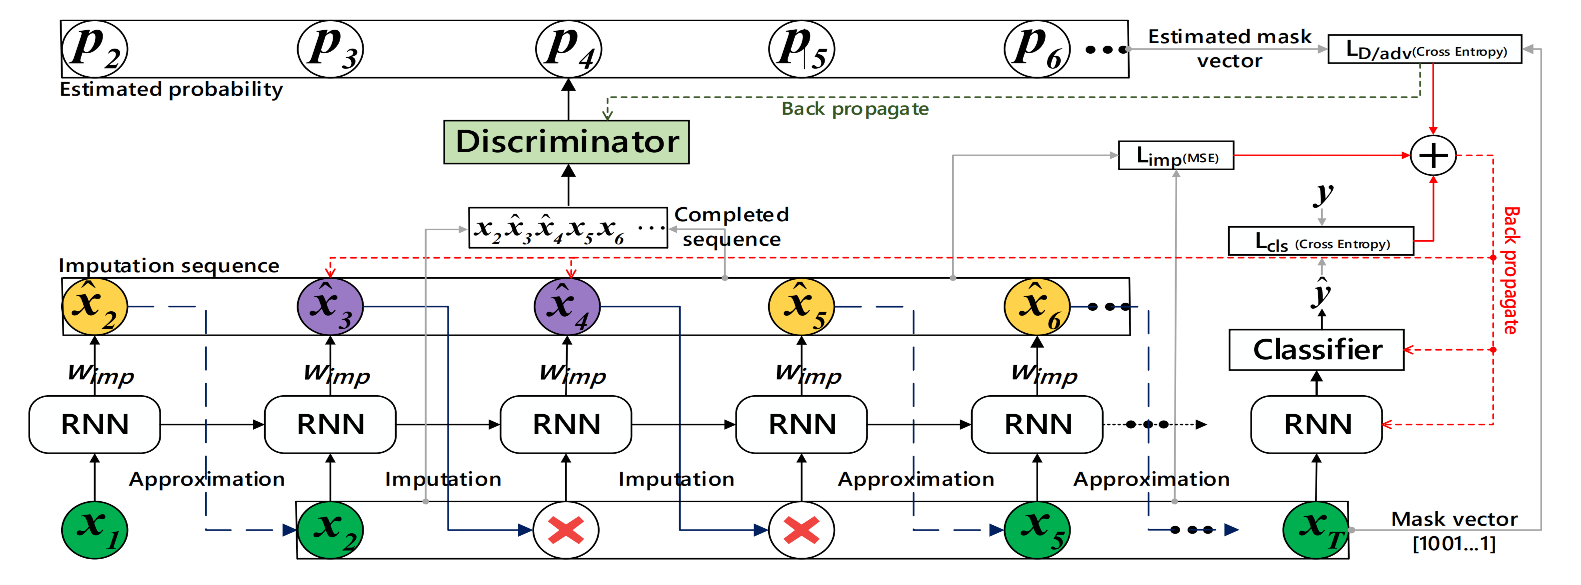
\includegraphics[width=1\textwidth]{ajrnn}
  \caption{The figure shows the proposed AJ-RNN framework. The green units represent revealed inputs, yellow for the output of approximated values, purple for the imputed values, and a red "X" for missing inputs. The dashed links represent the approximation training, while the solid links represent imputation. The discriminator receives a completed vector composed of revealed and imputed values as input, which provides a one-to-one supervisory signal for imputed values $\hat{x_3}$ and $\hat{x_4}$.}
  \label{fig:AJRNNrchitecture}
\end{figure}